\chapter{Dedykowana aplikacja w systemie Android}
\label{ch:aplikacja}
W tym rozdziale pokazana zostanie przykładowa aplikacja która współpracuję z rękawicą-kontrolerem. Aplikacja ta ma za zadanie wyświetlanie aktualnego stanu sensorów rękawicy oraz połączenia, a także prezentowanie tych danych. Pomimo możliwości wykorzystania wielu dostępnych platform do tworzenia animacji oraz środowisk wirtualnych, zdecydowano się na napisanie aplikacji na system Android wykorzystując do tego język Java. Aplikacja ta pozwala na wysoką mobilność, zagłębienie się w tematykę BLE, dzięki zaprogramowaniu własnego połączenia z serwisem udostępnianym przez rękawicę, a także łatwe zaznajomienie się z działaniem rękawicy nawet bez żadnej informacji dotyczącej jej obsługi. Rozdział ten przedstawia interfejs użytkownika, sposób komunikacji z rękawicą-kontrolerem a także opis używanego przez aplikację SDK o nazwie \textit{Google Sceneform}. Dołączony projekt firmy Google pozwala na importowanie modeli dłoni do aplikacji, prezentację ich a także odpowiada za animację na ekranie. W tym rozdziale zostaną pokazane zaimplementowane rozwiązania z którymi mierzą się twórcy kontrolerów, w szczególności przy wykorzystaniu nawigacji inercyjnej.

\section{Interfejs}
\label{sec:interface}
W niniejszej sekcji opisano interfejs wraz z jego elementami oraz ich funkcjonalność w ramach całej aplikacji. Aplikacja składa się z jednej aktywności o nazwie \textit{MainActivity} w ramach której został zaimplementowany układ zakładek, a konkretnie dwóch zakładek - dane oraz animacja. Zakładki te odpowiednio są uzupełnianie przygotowanymi fragmentami poprzez klasę \textit{SectionsPagerAdapter} oraz \textit{ViewPager}.W celu odpowiedniej obsługi fragmentów, aktywność ta musi implementować metody interfejsu \textit{OnFragmentInteractionListener}, które są zadeklarowane w klasach \textit{ModelRenderer} oraz \textit{GloveData}. Klasy te aby spełnić swoją funkcjonalność dziedziczą po klasie \textit{Fragment}~\cite{AndroidDoc}. W ten oto sposób zadeklarowano trzy klasy na podstawie których wyświetlany jest interfejs użytkownika, przedstawiony na rysunku~\ref{fig:ifce}. Metodę \textit{onCreate(Bundle)} przedstawia lsiting~\ref{lst:crt} na którym to widać krok po kroku sposób ładowania fragmentów w aktywności. Dwie ostatnie linie listingu pokazują wywołanie rejestracji odbiornika w celu otrzymywania informacji dotyczącego modułu Bluetooth wbudowanego w urządzenia na którym aplikacja jest uruchomiona. Oprócz wspominanych do tej pory klas, aplikacja korzysta również z dodatkowej klasy o nazwie \textit{VrGlove}, służącej do przechowywania informacji na temat kontrolera. Więcej informacji o tej klasie oraz o odbiorniku modułu Bluetooth zostanie przedstawionych w sekcji~\ref{sec:komunikacja}. 
\begin{lstlisting}[caption={Interfejs użytkownika.},captionpos=b,label={lst:crt},language = Java , frame = trBL , firstnumber = last , escapeinside={(*@}{@*)}]
    @Override
    protected void onCreate(Bundle savedInstanceState) {
        super.onCreate(savedInstanceState);
        setContentView(R.layout.activity_main);
        SectionsPagerAdapter sectionsPagerAdapter = new SectionsPagerAdapter(this, getSupportFragmentManager());
        ViewPager viewPager = findViewById(R.id.view_pager);
        viewPager.setAdapter(sectionsPagerAdapter);
        TabLayout tabs = findViewById(R.id.tabs);
        tabs.setupWithViewPager(viewPager);

        IntentFilter filter = new IntentFilter(BluetoothAdapter.ACTION_STATE_CHANGED);
        registerReceiver(mReceiver, filter);
    }
\end{lstlisting}


\begin{figure}[h]
\centering
	\begin{subfigure}[b]{0.45\textwidth}
	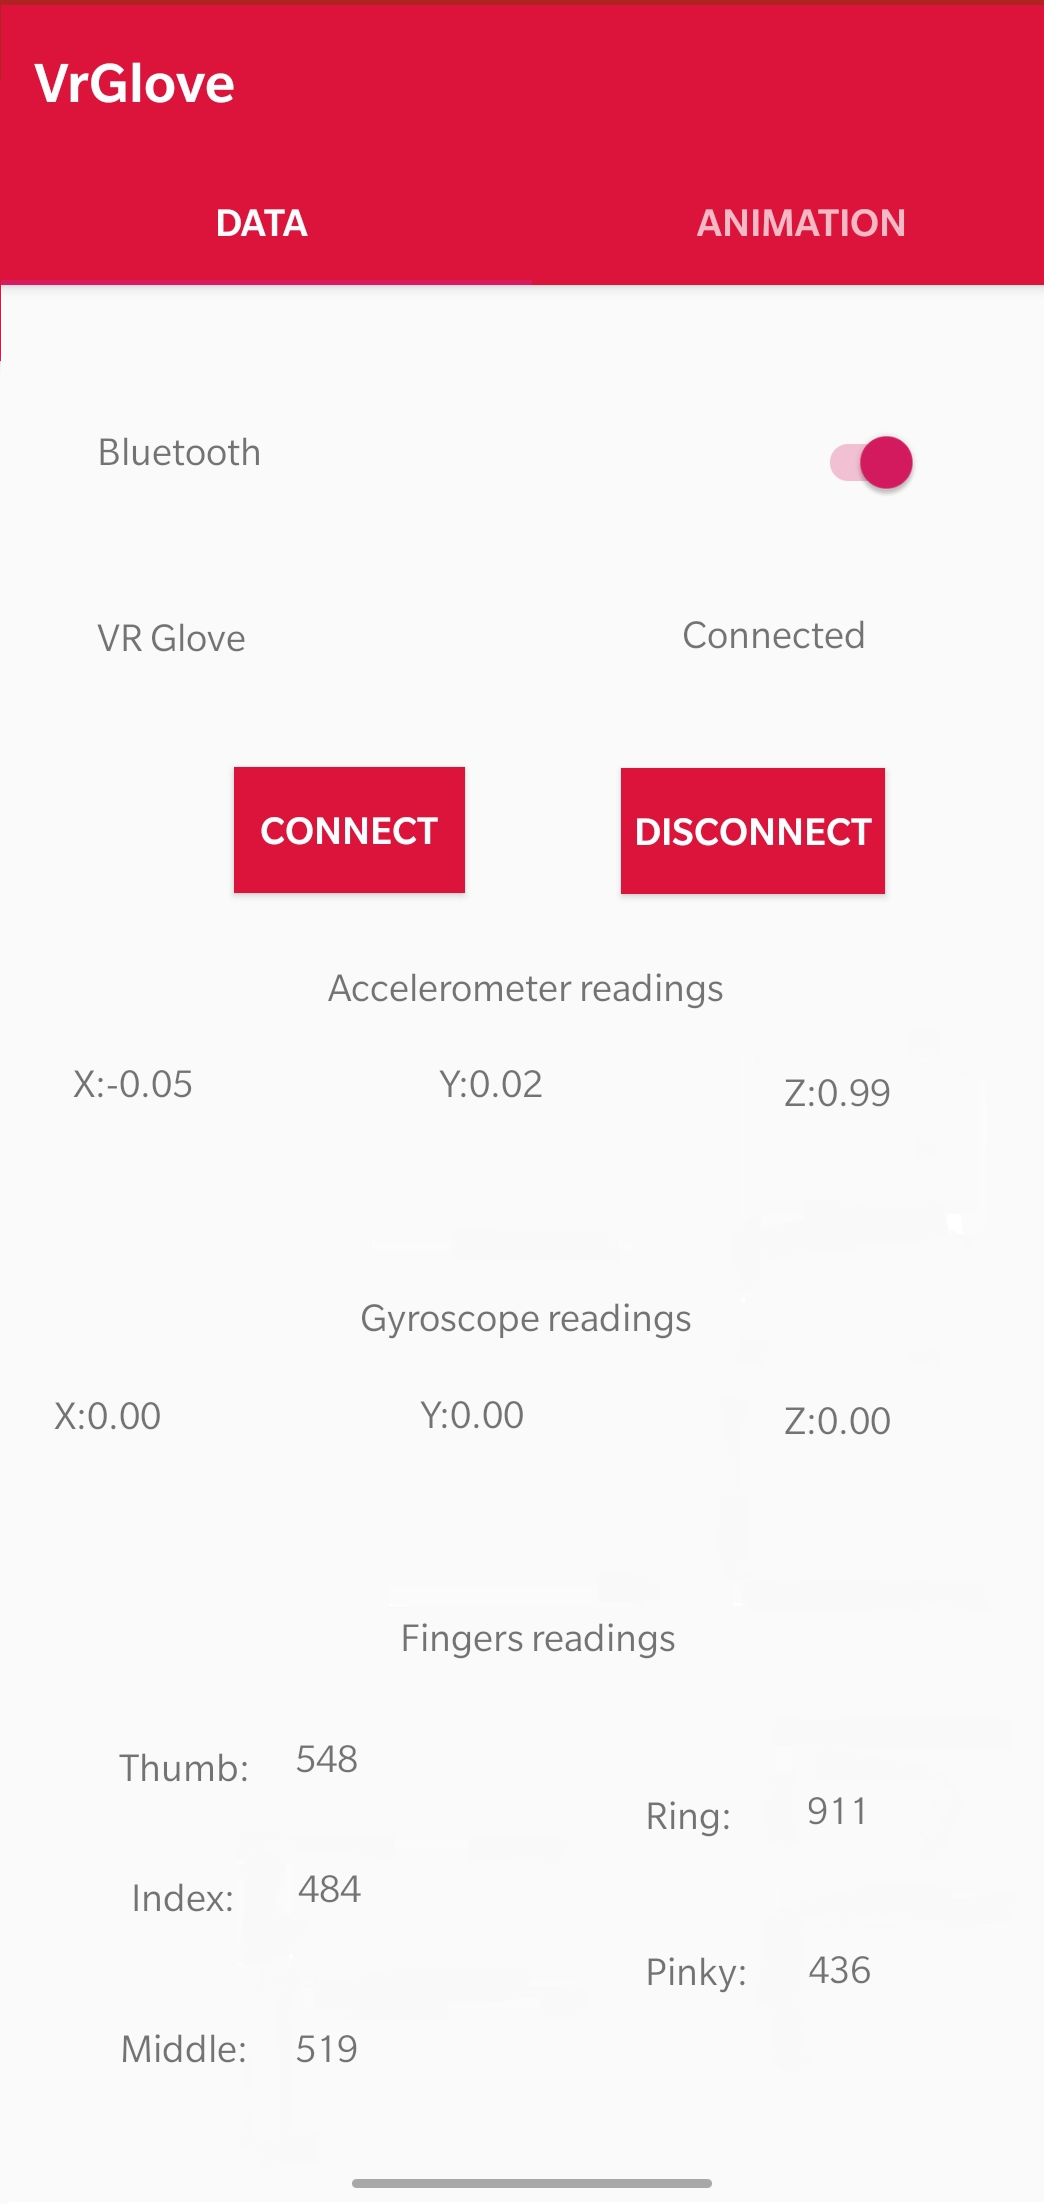
\includegraphics[width=\textwidth]{UI1}
	\caption{Fragment prezentujący dane}
	\label{fig:ifceDane}
	\end{subfigure}
	~
	\begin{subfigure}[b]{0.45\textwidth}
	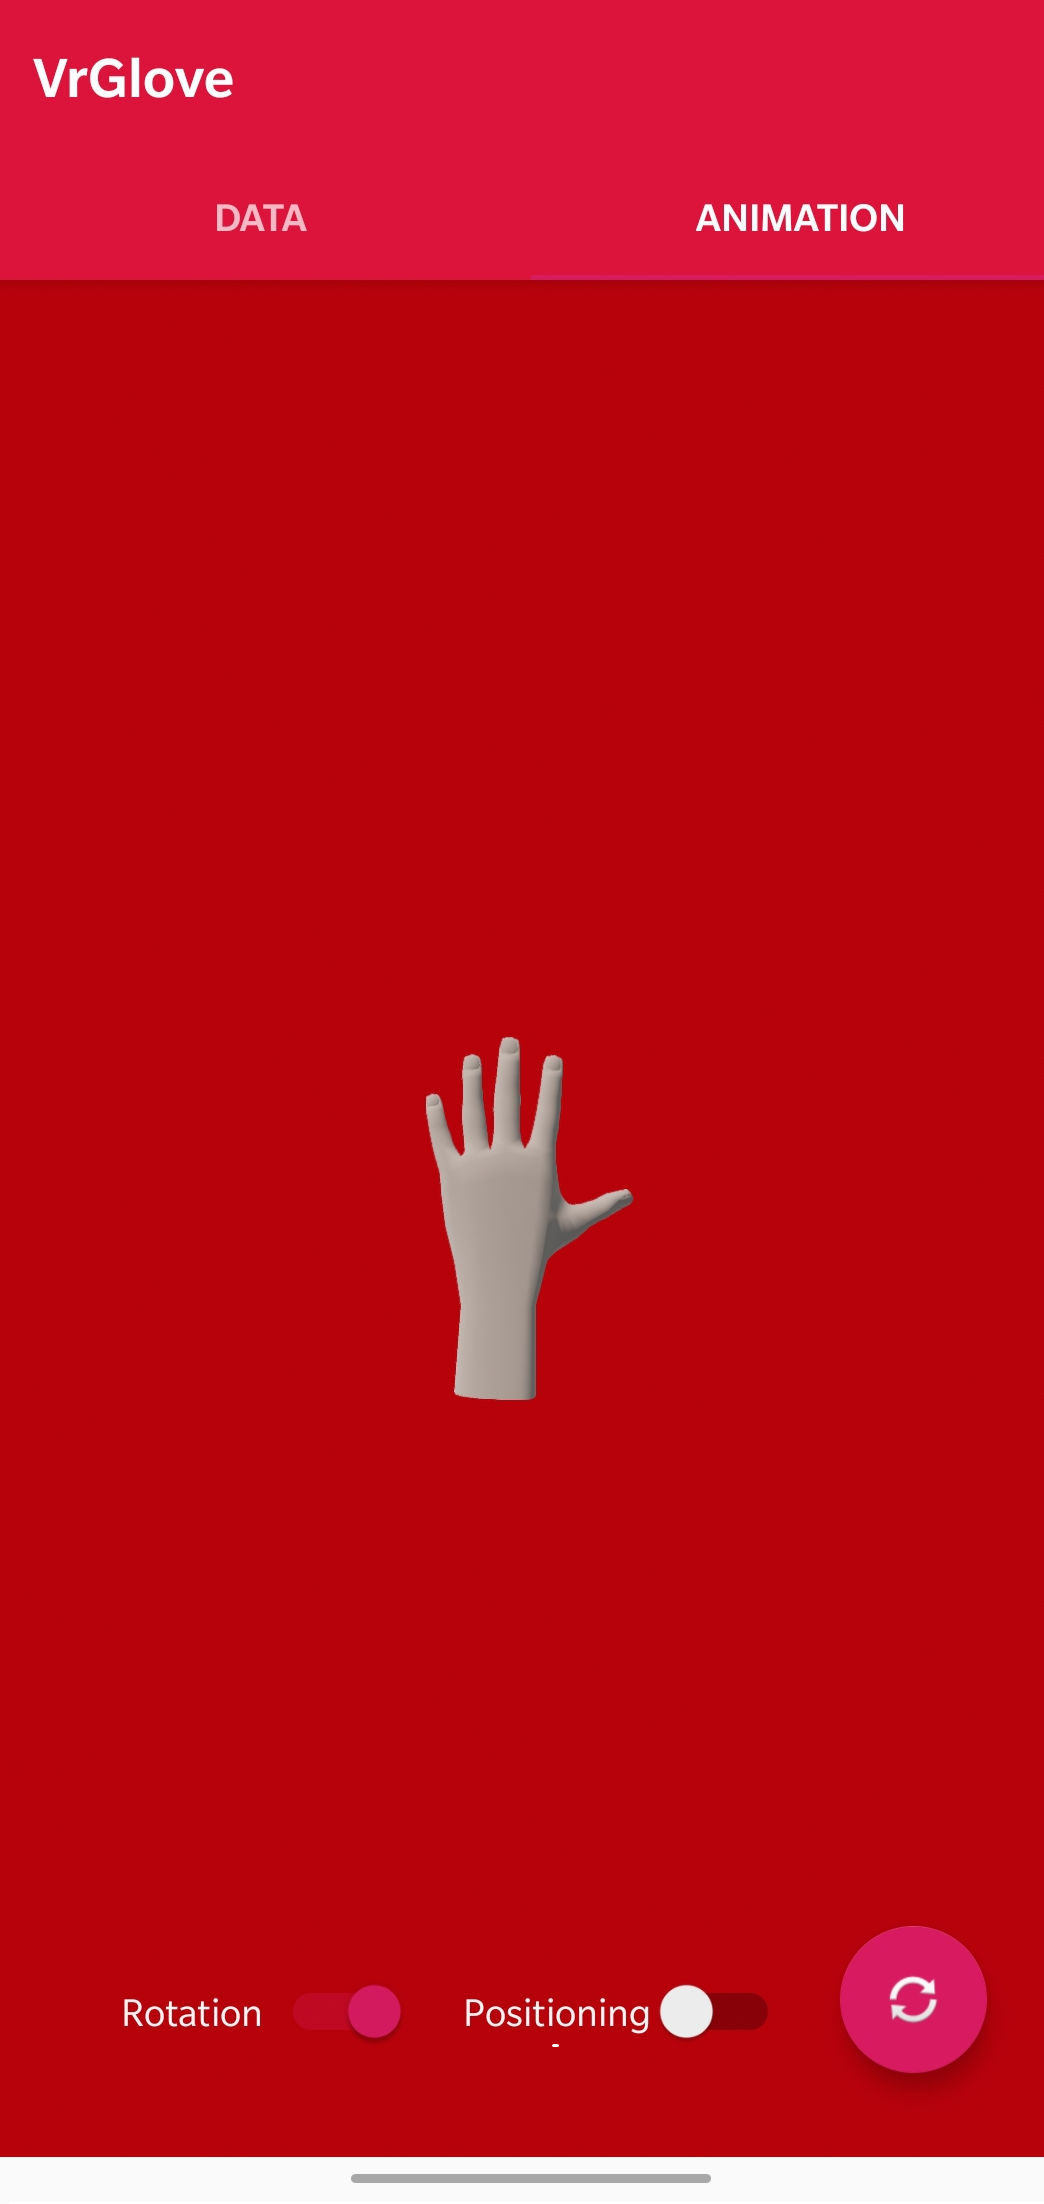
\includegraphics[width=\textwidth]{UI2}
	\caption{Fragment prezentujący animacje}
	\label{fig:ifceAnimacja}
	\end{subfigure}
\caption{Interfejs użytkownika}
\label{fig:ifce}
\end{figure}

Jak widać na~\cite{fig:ifceDane} rozpoczynając od góry widzimy informację dotyczącą obecnego stanu modułu Bluetooth w urządzeniu, wyrażanego poprzez przycisk przełącznika, pozwalający na włączenie/wyłączenie modułu bezpośrednio z poziomu aplikacji. Pod spodem Widnieje informacja o możliwości połączenia/statusie połączenia z kontrolerem opisana etykietą VR Glove. Etykieta ta przyjmuje następujące wartości:
\begin{itemize}
\item Włącz Bluetooth (ang. Turn On Bluetooth)
\item W trakcie włączania (ang. Turning On)
\item W trakcie wyłączania (ang. Turning Off)
\item Gotowy do połączenia (ang. Ready to connect)
\item W trakcie łączenia (ang. Connecting)
\item Połączony (ang. Connected)
\item W trakcie rozłączania (ang. Disconnecting)
\item Rozłączony (ang. Disconnected)
\end{itemize}
\label{itm:stany}
Pierwsze trzy stany możemy osiągnąć poprzez włączanie/wyłączanie modułu Bluetooth w urządzeniu. Stan gotowości do połączenia pokazuję się gdy moduł bluetooth został włączony i jest gotowy do połączenia z kontrolerem. Dwa przyciski znajdujące się poniżej etykiety, odpowiednio \textit{połącz (ang. Connect)} i \textit{rozłącz (ang. Disconnect)} pozwalają na połączenie z rękawicą-kontrolerem. Ostatnie cztery stany obrazują status połączenia z rękawicą, który możemy zmienić korzystając odpowiednio z przycisków. Poniżej znajdują się etykiety dotyczące sensorów kontrolera które są puste gdy aplikacja nie została jeszcze połączona z kontrolerem. Pola ta odpowiednio od góry reprezentują wartości zwracane przez akcelerometr i żyroskop jako wartości X,Y i Z, oraz wartości sensorów znajdujących się na palcach, z każdym sensorem mającym własną etykietę. Drugą częścią interfejsu prezentuje~\ref{fig:ifceAnimacja}, na której to widoczna jest lewa dłoń, znajdujące się na środku ekranu. Pozycja ta jest przyjmowana zanim kontroler zostanie podłączony. W dolnej części ekranu widzimy dwa przyciski przełączniki, służące do regulowania modelu, pozwalając decydować nam które elementy mają być brane pod uwagę podczas generowania animacji. Od lewej odpowiednio możliwe jest do zmiany branie pod uwagę orientacji kontrolera przy generowaniu modelu, następnie jego pozycji względem pozycji kalibracyjnej, oraz ostatni element tego interfejsu czyli FAB(z ang. Floating Action Button) - służący do ponownej kalibracji dłoni. Kalibracja ta jest również wywoływana przy każdej zmianie decyzji dotyczącej generowania rotacji bądź położenia. Pozycją kalibracyjną jest pozycja w której lewa dłoń na której znajduje się rękawica-kontroler, wraz ze wszystkimi palcami znajduję się w pozycji wyprostowanej, a kciuk wskazuje ciało użytkownika. Interfejs ten pozwala na szybkie połączenie się z kontrolerem a gdy tylko pierwsze dane zostaną przesłane do aplikacji, natychmiastowo obserwujemy pracę kontrolera na ekranie smart-fona. Warto zauważyć że po włączeniu aplikacji przełącznik orientacji jest włączony natomiast pozycjonowanie dłoni na ekranie wyłączone, w związku z czym animacja wyświetla się na środku ekranu. Do tej pory opisano wygląd i informacje elementów znajdujących się na ekranie, dalsza część tego rozdziału pokaże w jaki sposób wspomniane elementy działają od strony kodu źródłowego.

\section{Komunikacja}
\label{sec:komunikacja}
Opis interfejsu aplikacji pokazuje elementy które są wymagane oraz zaprogramowane w aplikacji. Pokazuje jakie dane są używana oraz w jakim celu wykorzystywane. Żeby jednak skorzystać z tych danych najpierw aplikacja musi zostać połączona z kontrolerem. W sekcji~\ref{subsec:mikrokontroler} powiedziano o wykorzystywaniu w tym celu połączenia BLE a o tym jak to jest obsługiwane przez prezentowaną aplikacje zostanie pokazane w części~\ref{subsec:ble}. Aby rozpocząć pracę z BLE przede wszystkim należy się upewnić że moduł Bluetooth w urządzeniu jest dostępny oraz włączony. W celu sprawdzenia dostępności modułu bluetooth w urządzeniu wykorzystywany jest plik \textit{AndroidManifest.xml}, w którym to zdefiniowano dostęp. Wszystkie wymagane pozwolenia pokazuje listing~\ref{lst:pozwolenia}.
	\begin{lstlisting}[caption={Wymagane pozwolenia dla aplikacji.},captionpos=b,label={lst:pozwolenia},language = Java , frame = trBL , firstnumber = last , escapeinside={(*@}{@*)}]
    <uses-permission android:name="android.permission.BLUETOOTH" />
    <uses-permission android:name="android.permission.BLUETOOTH_ADMIN" />
    <uses-permission android:name="android.permission.READ_EXTERNAL_STORAGE" />
    <uses-permission android:name="android.permission.CAMERA" />
\end{lstlisting}
Mając wymagany dostęp możemy sterować sensorem poprzez przycisk przełącznika. W kodzie programu wystarczy uzyskać do niego dostęp używając metody \textit{findViewById(int)} a następnie ustawić nasłuchiwacza kliknięć. Przyciski \textit{Połącz} oraz \textit{Rozłącz} są zdefiniowane w ten sam sposób. Aby wprowadzić zmiany w Bluetooth należy użyć klasy \textit{BluetoothAdapter}. Po pobraniu domyślnego adaptera jesteśmy w stanie określić jego stan. używając metod \textit{enable()} oraz \textit{disable()}. Sposób obsługi adaptera jest pokazany na listingu~\ref{lst:switchBT}. Zmiana ta wywołuję funkcję znajdującą się w klasie \textit{MainActivity} która reaguje na zmiany adaptera oraz ustawia jeden z pierwszych czterech statusów z listy~\ref{itm:stany} dla pola definiującego obecny stan połączenia. Skrócony listing~\ref{lst:status} pokazuje wywołanie tej funkcji dla przykładowego stanu adaptera. Ostatnie cztery stany wypunktowane w~\ref{itm:stany} pochodzą ze zmiany połączenia wywoływane poprzez wspomniane przyciski \textit{Połącz} oraz \textit{Rozłącz} które zostoną opisane w sekcji~\ref{subsec:ble}.
	\begin{lstlisting}[caption={Obsługa wbudowanego modułu Bluetooth.},captionpos=b,label={lst:switchBT},language = Java , frame = trBL , firstnumber = last , escapeinside={(*@}{@*)}]
switch (v.getId()){
            case R.id.switchBT:
            	Switch switchBT = v.findViewById(R.id.switchBT);
        		BluetoothAdapter mBluetoothAdapter = BluetoothAdapter.getDefaultAdapter();
                if (switchBT.isChecked()){
                    if (!mBluetoothAdapter.isEnabled()) {
                        mBluetoothAdapter.enable();
                    }
                }else{
                    if (mBluetoothAdapter.isEnabled()) {
                        mBluetoothAdapter.disable();
                    }
                }
                break;
                [...]
}
\end{lstlisting}
\begin{lstlisting}[caption={Zmiana statusu na podstawie adaptera bluetooth.},captionpos=b,label={lst:status},language = Java , frame = trBL , firstnumber = last , escapeinside={(*@}{@*)}]
private final BroadcastReceiver mReceiver = new BroadcastReceiver() {
        @Override
        public void onReceive(Context context, Intent intent) {
            final String action = intent.getAction();
            Switch tbBT= findViewById(R.id.switchBT);
            TextView tvStatus = findViewById(R.id.textView_vrGlove_status);
            if (action.equals(BluetoothAdapter.ACTION_STATE_CHANGED)) {
                final int state = intent.getIntExtra(BluetoothAdapter.EXTRA_STATE,
                        BluetoothAdapter.ERROR);
                switch (state) {
                    case BluetoothAdapter.STATE_OFF:
                        tbBT.setChecked(false);
                        tvStatus.setText("Turn on bluetooth");
                        break;
                    [...]
}                    
\end{lstlisting}

	\subsection{Obsługa połączenia Bluetooth Low Energy}
	\label{subsec:ble}
	Gdy poznano stan modułu Bluetooth, bez przeszkód można nawiązać połączenie. w tym celu wykorzystano przyciski sterujące połączeniem. Do przechowywania danych o połączeniu wykorzystywana jest klasa \textit{VrGlove}, w której zdefiniowano statyczne zmienne klasy \textit{BluetoothDevice} pozwalające na wybranie odpowiedniego urządzenia z puli dostępnych urządzeń w pobliży poprzez jego adres oraz \textit{BluetoothGatt} odpowiedzialnej za obsługę \textit{GATT} (z ang. Generic Attribute Profile) w androidzie. Listę dostępnych serwisów otrzymano deklarując zmienną implementującą listę klasy  \textit{BluetoothGattService}. W ten sposób w dowolnym miejscu programu można odwołać się do klasy kontrolera, sprawdzając jego stan a także uzyskać dane o jego udostępnionych serwisach. W ten oto sposób na listingu~\ref{lst:disconnect} pokazano dostęp do klasy rękawicy z nasłuchiwacza przycisku \textit{Rozłącz}. Fragment ten sprawdza czy istnieje aktualnie połączony serwis \textit{GATT} oraz czy jest on w stanie \textit{Połączony} wyrażony jako typ \textit{int} - 2. To właśnie na podstawie tego statusu są określane ostatnie cztery stany połączenia z rękawicą z listy~\ref{itm:stany}. Sposób zmiany statusu są bardzo zbliżone do listingu~\ref{lst:status}, różnica polega na wywołaniu odbiornika zmiany statusu połączenia z klasy \textit{BluetoothGattCallback} w przeciwieństwie do \textit{BroadcastReceiver} oraz zostaje wywołana metoda \textit{onConnectionStateChange} zamiast metody \textit{onReceive}. Jeżeli powyższe warunki są spełnione \textit{GATT} zostaje rozłączony~\cite{AndroidDoc}. 
\begin{lstlisting}[caption={Obsługa przycisku rozłącz.},captionpos=b,label={lst:disconnect},language = Java , frame = trBL , firstnumber = last , escapeinside={(*@}{@*)}]
case R.id.buttonDisconnect:
                if(VrGlove.getGatt() != null && VrGlove.getGattState() == 2 ){
                    VrGlove.getGatt().disconnect();
                }
                break;                    
\end{lstlisting}	
Ostatnia część którą opisano jest zarazem najważniejszą. Mowa o obsłudze przycisku \textit{Połącz}. Tak jak w przypadku przycisky \textit{Rozłącz}, najpierw sprawdzany jest status urządzenia, czyli czy adapter jest włączony oraz w przeciwieństwie do sprawdzania czy nasz serwis \textit{GATT} jest połączony, kod przycisku wykona się tylko wtedy gdy nie jest aktualnie nawiązane połączenie. Gdy warunki te są spełnione, zostaje pobrany adapter bluetooth oraz zostaje podjęta próba połączenia z urządzeniem przy użyciu klasy \textit{BluetoothDevice}, która otrzymuje zwracaną wartość metody \textit{getRemoteDevice(String)} wywołaną na adapterze bluetooth. W naszym przypadku jako parametr typu \textit{String}, zostaje podany adres \textit{D0:6B:F2:A7:95:03}, który jest adresem rękawicy-kontrolera z którym zostanie podjęta próba połączenia. Następnie zostaje stworzona nowa instancja klasy \textit{VrGlove}, której zostaje przekazana w parametrach wartość zmiennej typu \textit{BluetoothDevice} oraz aktualny widok na którym pracuje fragment. Posiadając te informacje rozpoczyna się kluczowy etap połączenia, mianowicie zostaje zainicjalizowana zmienna klasy \textit{BluetoothLeScanner}, poprzez wywołanie metody \textit{getBluetoothLeScanner()} na adapterze urządzenia. Metoda ta pozwala na wyszukiwanie urządzeń BLE znajdujących się w pobliżu, poprzez wywołanie metody \textit{startScan(ScanCallback)}, gdzie jako parametr zostaje podany stworzony skaner, oczekujący na pojawienie się urządzenia z wcześniej podanym adresem. Bardzo ważnym elementem jest zatrzymanie skanera gdy zostaje odnalezione urządzenie - co można osiągnąć poprzez wywołanie metody \textit{stopScan(ScanCallback)}. W ten oto sposób nawiązano połączenie pomiędzy urządzeniami a rezultat tego połączenie zostaje zapisany w postaci ustawienia serwisu \textit{GATT} w klasie \textit{VrGlove}. Opisane powyżej czynności są przedstawione na listingu~\ref{lst:connect}~\cite{AndroidDoc}. W ten oto sposób możemy kontrolować połączenie z kontrolerem z dedykowanej aplikacji. Ostatnim elementem poprawnego funkcjonowania jest przekazywanie danych w czasie rzeczywistym pomiędzy odbiornikiem a nadajnikiem, co zostanie pokazane w sekcji~\ref{subsec:dane}.
\begin{lstlisting}[caption={Kluczowe elementy przycisku \textit{Połącz} pozwalającego na połączenie z kontrolerem.},captionpos=b,label={lst:connect},language = Java , frame = trBL , firstnumber = last , escapeinside={(*@}{@*)}]
final BluetoothManager bluetoothManager =
                            (BluetoothManager) getActivity().getSystemService(Context.BLUETOOTH_SERVICE);
mBluetoothAdapter = bluetoothManager.getAdapter();
[...]
BluetoothDevice device = mBluetoothAdapter.getRemoteDevice("D0:6B:F2:A7:95:03");
new VrGlove(device,vw);                    
[...]
BluetoothLeScanner scanner = mBluetoothAdapter.getBluetoothLeScanner();
scanner.startScan(scanCallback);
[...]
scanner.stopScan(scanCallback);
gatt = VrGlove.getDevice().connectGatt(getActivity(),false,bluetoothGattCallback, TRANSPORT_LE);
VrGlove.setGatt(gatt);                                                           
\end{lstlisting} 

	\subsection{Pobieranie danych}
	\label{subsec:dane}
	Mając do dyspozycji informacja pozyskane w trakcie połączenia, które są przechowywane jako zmienne statyczne w klasie rękawicy, jesteśmy w stanie pozyskać dane które opisano w rozdziale~\ref{ch:rekawica}. W tym celu, po stronie aplikacji należy sprawdzić czy aktualnie jest nawiązane połączenie, co jak już zostało powiedziane oznacza serwis \textit{GATT} w stanie wyrażanym jako \textit{int = 2}.  Gdy potwierdzono połączenie, z klasy \textit{BluetoothGatt} zostaje wywołana metoda \textit{discoverServices()}, która jest wywoływana dopóki nie zostaną wykryte serwisy. Gdy tak się stanie, rezultat odnalezionych serwisów uzyskiwany jest poprzez metodę serwisu \textit{GATT} \textit{getServices()}. Mając dostęp do serwisów - w opisywanym przypadku wiemy z rozdziału dotyczącego rękawicy-kontrolera że jest to tylko jeden serwis, możemy pobrać cechy używając metody \textit{getCharacteristic(UUID)}, które ten serwis posiada. Cechy te zostały pokazane na listingu~\ref{lst:deklaracje}, oraz zostały przypisane im skrócone UUID wyrażone jako \textit{int} od $0x2101$ do $0x2103$, odpowiednio jako dane akcelerometru, żyroskopu oraz sensorów umiejscowionych na palcach. Implementacje algorytmu z typu \textit{int} do UUID pokazuje metoda \textit{convertFromInteger(int i)} na listingu~\ref{lst:UUID}~\cite{UUID}. 
	\begin{lstlisting}[caption={Zamiana zmiennej int na UUID.},captionpos=b,label={lst:UUID},language = Java , frame = trBL , firstnumber = last , escapeinside={(*@}{@*)}]
	private UUID convertFromInteger(int i) {
        final long MSB = 0x0000000000001000L;
        final long LSB = 0x800000805f9b34fbL;
        long value = i & 0xFFFFFFFF;
        return new UUID (MSB | (value << 32), LSB);
    }                                                       
\end{lstlisting}
Dla każdej cechy zostaje wywołana metoda \textit{readCharacteristic(BluetoothGattCharacteristic)}, która po sprawdzeniu warunków które są wymagane od każdej z cech dla prezentowanej aplikacji ustawia te cechy w trybie powiadomień - etap ten prezentuje listing~\ref{lst:notify}. Tryb powiadomień dla cechy oznacza że dane zostaną pobrane za każdym razem gdy zajdzie w nich jakaś zmiana. Ostatnią częścią jest pobranie deskryptora danej cechy. W ten sposób oprócz nawiązanego połączenia uzyskano dostęp do serwisów oraz cech reprezentowanych przez urządzenie z którym się połączono. Etap ten zaprezentowano na wycinku kodu~\ref{lst:characteristics}.

\begin{lstlisting}[caption={Uzyskanie dostępu do cech serwisu.},captionpos=b,label={lst:characteristics},language = Java , frame = trBL , firstnumber = last , escapeinside={(*@}{@*)}]     
if(VrGlove.getGattState() == 2){
	VrGlove.getGatt().discoverServices();                                                   
	[...]
	VrGlove.setServices(VrGlove.getGatt().getServices());
	for (int i = 0x2101;i<0x2104;i++){
    	mCharacteristic = VrGlove.getServices().get(2).getCharacteristic(convertFromInteger(i));
        readCharacteristic((mCharacteristic));
        BluetoothGattDescriptor descriptor = mCharacteristic.getDescriptor(convertFromInteger(0x2902)); 
        [...]
        VrGlove.getGatt().writeDescriptor(descriptor);
}
\end{lstlisting}

\begin{lstlisting}[caption={Ustawienie cechy w trybie powiadomień.},captionpos=b,label={lst:notify},language = Java , frame = trBL , firstnumber = last , escapeinside={(*@}{@*)}]     
private boolean readCharacteristic(final BluetoothGattCharacteristic characteristic) {
		// Check if GATT service exists        
        if(VrGlove.getGatt() == null) {
            Log.e(TAG, "ERROR: Gatt is 'null', ignoring read request");
            return false;
        }
        // Check if characteristic is valid
        if(characteristic == null) {
            Log.e(TAG, "ERROR: Characteristic is 'null', ignoring read request");
            return false;
        }
        // Check if this characteristic actually has READ property
        if((characteristic.getProperties() & PROPERTY_READ) == 0 ) {
            Log.e(TAG, "ERROR: Characteristic cannot be read");
            return false;
        }
        VrGlove.getGatt().setCharacteristicNotification(characteristic, true);
        return true;
    }                                                      
\end{lstlisting}

Ważnym elementem tego procesu jest odczytywanie cech pojedynczo, z racji tego że serwis \textit{GATT} obsługuję połączenie tylko z jedną cechą jednocześnie, co oznacza że gdyby spróbowano pobrać następną cechę, podczas gdy połączenie nie zostało zakończone z poprzednią cechą - połączenie to zostanie nadpisane. Obsługę połączenia z cechą zapewnia nadpisanie metody \textit{onCharacteristicChange(BluetoothGatt, BluetoothGattCharacteristic)} wywoływaną  z klasy \textit{BluetoothGattCallback}. Kod został napisany właśnie w tej metodzie ze względu na tryb w jaki cechy zostały ustawione, czyli tryb powiadomień. Dzięki temu funkcja ta zostaje wywołana za każdym razem gdy obserwowane cechy zostaną w jakiś sposób zmienione. W zależności od rozpoznanej cechy, wywoływana jest metoda zmieniające aktualny zestaw danych w klasie kontrolera, co pokazuje listing~\ref{lst:findChar}. Następnie funkcje klasy \textit{VrGlove} przypisują zmiennym odpowiadającym sensorom nowe dane oraz dokonują ich konwersji z tablicy typu \textit{byte} do typu \textit{float}. Dane te po obróbce są przypisywane odpowiednim polom w interfejsie użytkownika. Pobieranie danych polega na wycinaniu z tablicy informacji kolejnych 4 bajtów, co jest równoznaczne jednej zmiennej typu \textit{float}. Ważne dla konwersji jest również sposób w jaki dane zostają zamienione - w tym przypadku używana jest notacja \textit{LITTLE\_ENDIAN}. Wykonane kroki pokazuje listing~\ref{lst:setChar} dla odczytu pierwszej wartości z tablicy danych żyroskopu. Proces ten należy wykonać dla wszystkich wartości w danej cesze oraz odpowiednio dla każdej z pobieranych cech~\cite{AndroidDoc}.
\begin{lstlisting}[caption={Odczytywanie danych cechy.},captionpos=b,label={lst:findChar},language = Java , frame = trBL , firstnumber = last , escapeinside={(*@}{@*)}]     
 if(characteristic.getUuid().equals(convertFromInteger(0x2101))){
	VrGlove.setAccReadings(value);
}else if (characteristic.getUuid().equals(convertFromInteger(0x2102))){
	VrGlove.setGyroReadings(value);
}else if(characteristic.getUuid().equals(convertFromInteger(0x2103))){
	VrGlove.setFingersReadings(value);
}else{
	Toast.makeText(getActivity(),"Unknown characteristic",Toast.LENGTH_SHORT);
}                                                   
\end{lstlisting}

\begin{lstlisting}[caption={Przypisywanie danych pozyskanych z cech, do zmiennych w aplikacji.},captionpos=b,label={lst:setChar},language = Java , frame = trBL , firstnumber = last , escapeinside={(*@}{@*)}]     
     static void setGyroReadings(byte[] gyroReadings) {
        VrGlove.gyroReadings = gyroReadings;
        getGyroReadings();
    }      
    
     private static void getGyroReadings() {
        TextView x = vw.findViewById(R.id.textView_gyr_X);
        Float[] data = new Float[3];
        
        float f = ByteBuffer.wrap(gyroReadings,0,4).order(ByteOrder.LITTLE_ENDIAN).getFloat();
        data[0] = f;
        x.setText(String.format("X:%.2f",f));
      	[...]

        dataSet.put("Gyro",data);
        setmIsStateChanged(true);
    }                                      
\end{lstlisting}

W tej sekcji został pokazany sposób połączenia aplikacji z kontrolerem, oraz sposób w jaki po ustanowieniu połączenia dane zostają przekazane i obrabiane. W ten sposób fragment \textit{GloveData}, odpowiedzialny za prezentację interfejsu pokazanego na rysunku~\ref{fig:ifceDane} kończy swoje działanie. Na podstawie tych danych fragment \textit{ModelRenderer} jest w stanie wygenerować drugą część interfejsu która zostanie teraz opisana.

\section{Google Sceneform SDK}
\label{sec:sceneform}
Jak widać na zdjęciu interfejsu~\ref{fig:ifceAnimacja}, drugi fragment prezentuje dłoń, której pozycja, orientacja oraz kształt zmienia się w czasie rzeczywistym. Aby to osiągnąć zdecydowano się na wybór SDK udostępnionego od \textit{Google}, służącego do renderowania realistycznych scen w aplikacjach na androida. Pomimo oryginalnego zastosowania służącego do budowania aplikacji AR (z ang. Augmented Reality), zestaw narzędzi został rozbudowany do obsługi aplikacji spoza tej dziedziny. W ten oto sposób, bez znajomości OpenGl otrzymano dostęp między innymi do narzędzi, obsługujących scenę na której renderowane są obrazy, a także wtyczki do Android Studio, pozwalającej na importowanie modeli 3D do aplikacji w prosty sposób. Wtyczkę dodano do środowiska programistycznego poprzez wyszukanie w menu \textit{Wtyczki}, wtyczki o nazwie \textit{Google Sceneform Tools (Beta)}. W ten oto sposób po kliknięciu prawym przyciskiem myszy na model znajdujący się w drzewie projektu, pojawia się opcja \textit{zaimportuj model}, tworząca dwa pliki na podstawie których \textit{Sceneform} generuje model na ekranie: \textit{.sfa} oraz \textit{.sfb}. Gdy zainstalowano wtyczkę, należy pobrać z oficjalnego linku do strony projektu Github foldery zawierające SDK. Foldery te należy dodać do projektu, które od teraz są jego częścią. Szczegółowy opis jak przeprowadzić ten proces znajduję się w dokumentacji SDK. Ważną informacją dotyczącą tego projektu jest fakt że w Marcu 2020 roku, repozytorium zostało zarchiwizowane, a Google nie przewiduje dalszych prac nad projektem~\cite{sceneform}. 
	\subsection{Model ręki}
	\label{subsec:model}
	Model ręki zastosowany w projekcie został stworzony przez 3DHaupt, i jest udostępniony do użytkowanie za darmo w celach edukacyjnych, oraz do celów niekomercyjnych. Model został wykonany w programie \textit{Blender}, i posiada w pełni użytkowy szkielet, dzięki któremu można ustawić dłonie w dowolnej pozycji~\cite{hands}. Aplikacja obsługuje jedynie rękawice-kontroler przeznaczoną dla lewej dłoni, w związku z czym tylko ta część modelu została zachowana. Korzystając z programu blender, zmodyfikowany szkic został zapisany w formacie \textit{.obj}, a następnie umieszczony w folderze aplikacji o nazwie sampledata. Oprócz modelu dłoni z wyprostowanymi palcami, pokazanego na rysunku~\ref{fig:ifceAnimacja}, zostały przygotowane dodatkowe cztery modele. Modele te zostały pokazane na rysunku~\ref{fig:modele}.
\begin{figure}[h]
\centering
	\begin{subfigure}[b]{0.22\textwidth}
	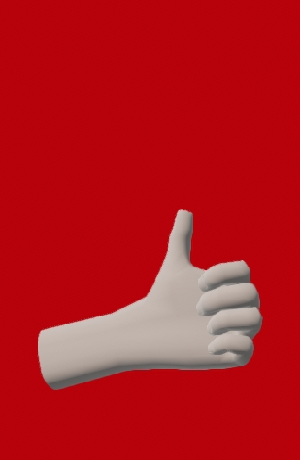
\includegraphics[width=\textwidth]{OK}
	\caption{Model: OK}
	\label{fig:modelOk}
	\end{subfigure}
	~
	\begin{subfigure}[b]{0.22\textwidth}
	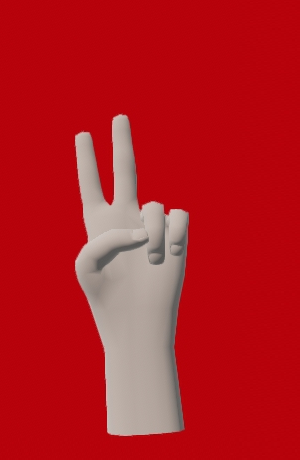
\includegraphics[width=\textwidth]{PEACE}
	\caption{Model: Pokój}
	\label{fig:modelPeace}
	\end{subfigure}
	~
	\begin{subfigure}[b]{0.22\textwidth}
	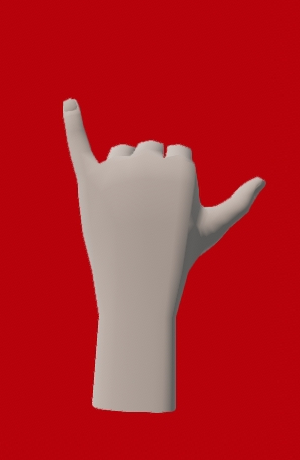
\includegraphics[width=\textwidth]{MAHALO}
	\caption{Model: Mahalo}
	\label{fig:modelMahalo}
	\end{subfigure}
	~
	\begin{subfigure}[b]{0.22\textwidth}
	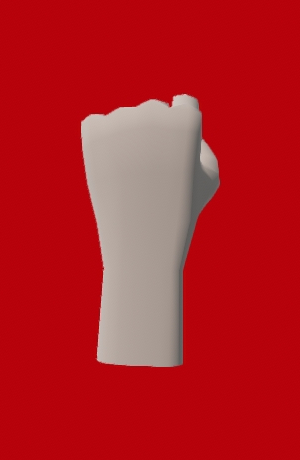
\includegraphics[width=\textwidth]{FIST}
	\caption{Model: Pięść}
	\label{fig:modelFist}
	\end{subfigure}
\caption{Modele animacji dłoni.}
\label{fig:modele}
\end{figure}

	
	
	\subsection{Dodawanie nowego modelu}
	\label{subsec:nowyModel}
	
	
	
	\subsection{Rozpoznanie i animacja modelu}
	\label{subsec:rozpoznanie}
	
	
	
	
	\subsection{Rotacja}
	\label{subsec:rotacja}
	
	
	
	\subsection{Przesunięcie}
	\label{subsec:przesuniecie}	
	
	
	
	\subsection{Kalibracja}
	\label{subsec:kalibracja}
	
	

